\subsection{MetaQC}
MetaQC package provides an objective and quantitative tool to help determine the inclusion/exclusion of studies for meta-analysis. More specifically, MetaQC provides users with six quantitative quality control (QC) measures: including IQC, EQC, AQCg, CQCg, AQCp and CQCp. Details of how each measure is defined and computed can be found in the Manuscript. In addition, visualization plots and summarization tables are generated using principal component analysis (PCA) biplots and standardized mean ranks (SMR) to assist in visualization and decision. Detailed information can be found in the ``MetaQC" package in the metaOmics software suite (\url{https://github.com/metaOmics/MetaQC}). The test data used to demo the ``MetaQC" package here is merged from eight prostate cancer studies and 50\% mean filtering and 50\% variance filtering. 
Detailed descriptions of these studies can be found in Table~\ref{tab:realDataProstate}. 

\subsubsection{Procedure}

\begin{figure}[H]
\begin{center}
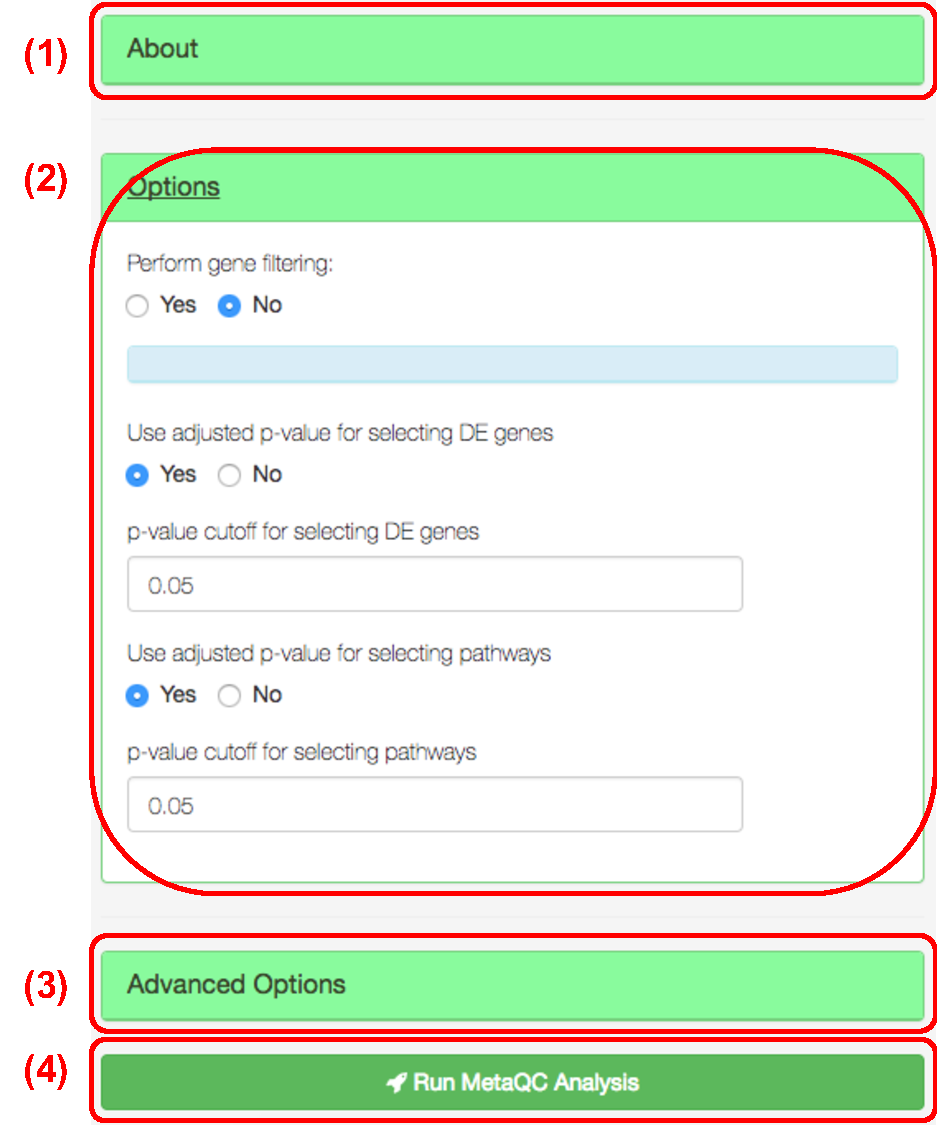
\includegraphics[scale=0.5]{./figure/metaQC/metaQCoption.pdf}
\caption{``MetaQC" options}
\label{fig:MetaQCoption}
\end{center}
\end{figure}

There are three main options available for the ``MetaQC" package as shown in Figure~\ref{fig:MetaQCoption}. 

\begin{steps}
\item \textbf{Options:}
Under the drop-down menu ``options" ({\color{red}(2)} in Figure~\ref{fig:MetaQCoption}),
users can specify whether to 

\begin{itemize}
\item perform gene filtering. Gene filtering is suggested to reduce computational cost. Once ``Yes" is chosen for gene filtering, users are further asked to specify the filtering cutoffs by mean or by variance like in merging step. In the demo example, the merged data have already had gene filtering, no further filtering is performed. 
\item users need to specify the approach (either by raw p-value or FDR) and cutoff to select potentially DE genes needed in the computation of IQC, EQC, AQCg and CQCg.
\item users need to specify the approach (either by raw p-value or FDR) and cutoff to select potentially enriched pathways needed in the computation of AQCp and CQCp.
\end{itemize}

\item \textbf{Advanced options:}

Under the drop-down menu ``Advanced Options" ({\color{red}(3)} in Figure~\ref{fig:MetaQCoption}), users are allowed to tune other parameters of MetaQC.
In particular, it includes the selection of pathways by pathway size and the number of permutations to run to obtain the six measures. A detailed list of all options available for the package can be found at the end of the section. 
However, this is optional and users are suggested not to modify the option setting in this section without knowing the method. 

\item \textbf{Run MetaQC Analysis:}

Once all the above options are specified, users can click on {\color{red}(4)} ``Run MetaQC Analysis" to implement the tool. 

\end{steps}


\textbf{Complete List of Options:} 

\begin{enumerate}
  \item Options
  \begin{itemize}
     \item Perform gene filtering: If yes: cut lowest percentile by mean, cut lowest percentile by variance. 
     \item Use adjusted p-value for selecting DE genes
     \item p-value cutoff for selecting DE genes
     \item Use adjusted p-value for selecting pathways
     \item p-value cutoff for selecting pathways
    \end{itemize}
   \item Advanced Option (**Optional): 
        \begin{itemize}
      \item Pathway min gene size
      \item Pathway max gene size
      \item Number of permutations
    \end{itemize} 
  \item Run MetaQC Analysis
\end{enumerate}
   

\subsubsection{Results}


\begin{figure}[H]
\begin{center}
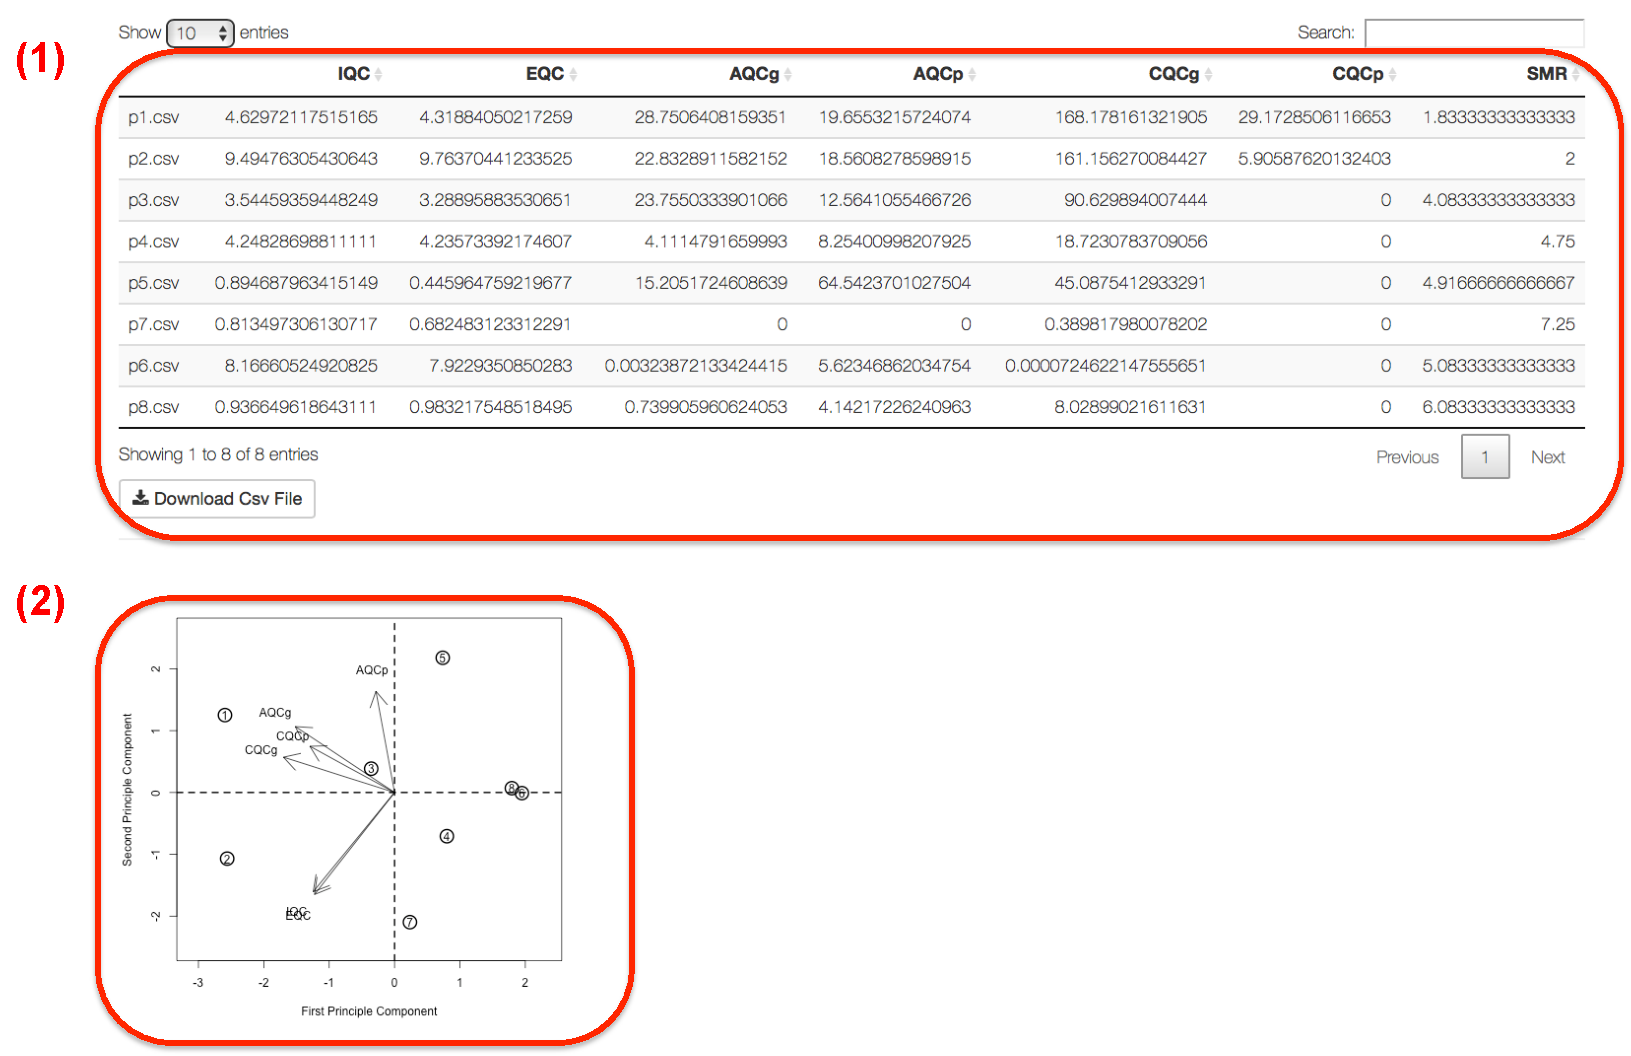
\includegraphics[scale=0.7]{./figure/metaQC/metaQCresult.pdf}
\caption{``MetaQC" Results}
\label{fig:MetaQCresult}
\end{center}
\end{figure}

We applied MetaQC on the eight prostate cancer datasets.
After performing merging of the eight datasets and filtering out 50\% genes by mean and 50\%  by variance, 1060 genes remained for the MetaQC analysis.
As shown in Figure \ref{fig:MetaQCresult}, there are {\color{red} (1)} a summary table of MetaQC results as well as {\color{red} (2)} a PCA biplot generated. The table includes seven columns, with the first six columns corresponding to the six quantitative quality control measures of all studies (a larger value indicates a better quality) and the seventh column is the rank summary statistics of all the six quality measures (a lower rank indicates a better quality). Users can download the full table as a csv file by clicking on ``Download Csv File". In addition to the tabular results, ``MetaQC" also generated a PCA biplot based on the six quality control measures, where the circled number is the study index and arrows indicate different measures. Generally, studies with larger SMR values, and studies more off from the other studies and a majority of the measures are considered lower quality. In this case, the 7th and the 8th studies have relatively poorer quality. Both tabular summary and biplot are automatically saved to the working directory. 


